\documentclass[landscape]{sciposter}

% edit pointsize, width, height, and fontsize parameters as needed
% DO ensure that values in the \special commands match!
\renewcommand{\papertype}{custom}
\renewcommand{\sectionsize}{\large}
\renewcommand{\fontpointsize}{25pt}
\setlength{\paperwidth}{36in}
\setlength{\paperheight}{24in}
\renewcommand{\setpspagesize}{
\ifthenelse{\equal{\orientation}{landscape}}{
\special{papersize=36in, 24in}
}{\special{papersize=24in, 36in}
}
}

% Setting correct textlenghts that are compatible with paper size.
\setmargins[2cm]


%\renewcommand{\subsectionsize}{\large \textcolor{\SectionCol}}
%\usepackage[spanish]{babel}
% or whatever

%% Define Lean to be the default language for Listing
\usepackage[utf8x]{inputenc}
\usepackage{color}
\definecolor{keywordcolor}{rgb}{0.7, 0.1, 0.1}   % red
\definecolor{commentcolor}{rgb}{0.4, 0.4, 0.4}   % grey
\definecolor{symbolcolor}{rgb}{0.0, 0.1, 0.6}    % blue
\definecolor{sortcolor}{rgb}{0.1, 0.5, 0.1}      % green
\usepackage{listings}
\def\lstlanguagefiles{lstlean.tex}
\lstset{language=lean,frame=lines,basicstyle=\small}

% Change to a font that has all the glyphs. This option necessitates
% XeLaTeX or LuaLaTeX as the compiler engine.
\usepackage{fontspec}
\setmonofont{DejaVu Sans Mono}[Scale=MatchLowercase]


\usepackage{amsmath}
\usepackage{amssymb}
\usepackage{graphicx}
\usepackage{amsmath,amsthm,amssymb}
\usepackage{multicol}
\usepackage{listings}
\usepackage{enumerate, wrapfig}
\usepackage{colortbl}
\usepackage[export]{adjustbox}
\usepackage{enumitem}
\setlist[enumerate]{
  leftmargin=2cm,
  before=\setlength{\listparindent}{-\leftmargin},
}





\newtheorem{thm}{Theorem}%[section] % uncomment [section] to number within section
\newtheorem*{thm*}{Theorem}
\newtheorem{lem}[thm]{Lemma}
\newtheorem{cor}[thm]{Corollary}
\newtheorem{prop}[thm]{Proposition}
\newtheorem{rem}[thm]{Remark}
\newtheorem{cond}[thm]{Condition}
\newtheorem*{namedtheorem}{Theorem}
\newtheorem{ex}{Example}
\newtheorem*{definition}{Definition}
\newtheorem{env}[thm]{Variation}
\renewcommand {\theequation}{\arabic{section}.\arabic{equation}}
\newcommand{\R}{\ensuremath{{\Bbb R}}}

%Lines 54-73 define box theorem. You can do similar things to put boxes around conjectures, corollaries, ect, or use the mdframe to just create a box
\usepackage[framemethod=TikZ]{mdframed}

\mdfdefinestyle{MyFrame}{linecolor=orange,
    outerlinewidth=2pt,
    roundcorner=50pt,
    innertopmargin=\baselineskip,
    innerbottommargin=\baselineskip,
    innerrightmargin=15pt,
    innerleftmargin=15pt,
    backgroundcolor=white}


\mdtheorem[style=MyFrame]{MDtheorem}{Theorem}
\newcommand*{\Title}{}
\newenvironment{boxthm}[1][]{%
\refstepcounter{thm}
    \ifstrempty{#1}{\begin{MDtheorem}}%
    {\begin{MDtheorem}[(#1)]}
}{%
    \end{MDtheorem}%
}%

%\definecolor{BoxCol}{rgb}{0.9,0.9,0.9}
% uncomment for grey background to \section boxes
% for use with default option boxedsections

\definecolor{BoxCol}{rgb}{.06,.16,.28}


\definecolor{SectionCol}{rgb}{1,1,1}

\definecolor{blue}{rgb}{0,0,1}
\definecolor{orange}{rgb}{.93,.29,0.1}
\definecolor{white}{rgb}{1,1,1}

\newtheorem{Features}{Features}

\usepackage{listings}
\usepackage{color}

\definecolor{dkgreen}{rgb}{0,0.6,0}
\definecolor{gray}{rgb}{0.5,0.5,0.5}
\definecolor{mauve}{rgb}{0.58,0,0.82}




%%%%%%%%%%%%%%%%%%%%%%%%%%%%%%%%%%%%%%%%%%%%%
%title
%%%%%%%%%%%%%%%%%%%%%%%%%%%%%%%%%%%%%%%%%%%%%
\title{\hspace{-5cm}Theorem Proving In Lean}
% \author[Faculty Advisor: ]{Dr. Philipp Hieronymi}
\author{Faculty Advisor: Dr. Philipp Hieronymi\\Graduate Mentors: Vaibhav Karve, Scott Harman, Eion Blanchard\\
Nikil Ravi, Kyle Thompson, Fenglong Zhao, Tianfan Xu, Joel Schargorodsky, Noble Wulffraat}

% insert correct institute name
%\institute{University of Illinois at Urbana-Champaign}
%\email{}  shows author email address below institute

%\date is unused by the current \maketitle

%%%%%%%%%%%%%%%%%%%%%%%
% Logo for Poster
%%%%%%%%%%%%%%%%%%%%%

\leftlogo[.7]{igl-logo-small.png} % defines logo to left of title (with scale factor)
\rightlogo[.6]{imark.png} % same but on right

%%%%%%%%%%%%%%%%%%%
% Start of document
%%%%%%%%%%%%%%%%%%%
\begin{document}
%%%%%%%%%%%%%%%%%%%%%%
%% Poster Set up
%%%%%%%%%%%%%%%%%%%%%%%
\conference{IGL Poster Session Fall 2020}% you can change this for other conferences

\maketitle
\vspace{-3ex}
\begin{multicols}{4}  % sets up 3 column poster



%%%%%%%%%%%%%%%%%%%%%%
%% Start of First Column
%%%%%%%%%%%%%%%%%%%%%%%
%Sections have a color box around them. Remove the * if you want to number your sections
\section*{Introduction}

A theorem prover is a program that takes a statement and verifies or decides (i.e., proves or disproves) it. Given that most proof methods can be reduced to a set of axioms and associated rules, we can use theorem provers to either prove that a statement is correct, or verify the correctness of a given proof. Because of the reliability and efficiency that theorem provers provide, they can be useful in many contexts in mathematics and beyond.\\

\section*{The Lean Theorem Prover}

Lean is a software used for theorem proving and formal verification. It aims to bridge the gap between interactive theorem proving, which focuses more on verifying proofs down to the axioms, and automated theorem proving, which attempts to find a proof for a given statement.\\

As a very basic example of some Lean code, consider the following definition of an even number, written using Lean:\\

\begin{lstlisting}
def even (n : ℕ) : Prop := ∃ d, n = 2 * d
\end{lstlisting}

In order to now 'prove' that a given number, say \(6\), is even, we would have to convince Lean that the number \(6\) satisfies the definition of an even number given above. One way to do this is:\\

\begin{lstlisting}
lemma even_zero : even 6 :=
begin
  unfold even,
  use 3,
  norm_num,
end
\end{lstlisting}

The lines of code between begin and end consist of tactics- these are similar to statements in a proof written by a human mathematician. Informally, 'unfold even' tells Lean to read the definition of an even number, 'use 3' asks Lean to use 3 as d in the definition, and 'norm$\_$num' is a tactic in Lean that can be used here to verify that 2 * 3 = 6.



\section*{Project Description}
The aim of this project is to use Lean to formalize ideas in first-order logic and model theory. We focus on aspects including but not limited to: languages, structures, embeddings between structures,
variables, terms, sentences, models and o-minimality.\\ \\Definitions for each of the above notions were written using Lean, and then relevant theorems and lemmas were stated with a formal proof in Lean. We have also included many examples for most of our definitions.

\section*{Languages and Structures}

We used the definition of language and structure from Marker's \textit{Model Theory}.

\begin{definition}[Language]

A language L is a set of constants, function symbols and relation symbols.

\end{definition}

\textbf {Things need to know}: \\
1.Constants of a language are simply its 0-ary functions. \\
2.Function and relation symbols have the arity at least 1. \\
3.We can specify one language by its function, relation, and constant.

\textbf{Examples for language}: \\
\textbf{A simple example of language in Lean}
\begin{lstlisting}
/-- The language of ordered sets is the language or sets with a binary ordering relation {$\textless$}.-/
def ordered_set_lang : lang := {R := $\lambda$ n : ℕ, if n=2 then                                                        unit else empty,
                                            F :=  function.const $\mathbb{N}$ empty}
\end{lstlisting}

Explanation : A brief example that has a binary ordering relation "<" and only when n = 2, it will do this binary operation and give a unit(a set with one element).\\

\textbf{Another Example of language in Lean}\\
\begin{lstlisting}
/-- A monoid is a {x,1}-structure which satisfies the identities
   1. u x (v x w) = (u x v) x w
   2. u x 1 = u
   3. 1 x u = u. -/

def monoid_lang : lang := {F := $\lambda$ n : $\mathbb{N}$,
                                        if n = 0 then unit else
                                        if n = 2 then unit else empty
                                      R := function.const $\mathbb{N}$ empty}
\end{lstlisting}
Explanation : This example is language for monoid.  For the function symbol, if n = 0, then just return a constant number in the unit set. And if n = 2, the 'x' operator works, which is a binary function symbol and it will also return a number, which we know is actually the result of the multiplication. In other cases, it will return empty.


Now we will give the definition of structure in mathematical way and
lean language. Note that languages will obtain their meanings only
when expressed in proper structure.

\textbf{Definition:} Let \textit{L} be a language. An \textit{L-structure} is a pair $\mathfrak{A} = (A,(Z^\mathfrak{A})))$, where $Z \in L$. \\
\textbf{Notation:} \begin{enumerate}
    \item    A is a non-empty set,the domain of $\mathfrak{A}$.
    \item    $Z^\mathfrak{A}\in A$ if Z is a constant.
    \item    $Z^\mathfrak{A} : A^n \longrightarrow A$ if Z is an n-ary function symbol.
    \item    $Z^\mathfrak{A} \subseteq A^n$ if Z is an n-ary relation symbol.\\
    We call $Z^\mathfrak{A}$ the $\mathfrak{A}$-interpretation of Z.
\end{enumerate}

\begin{lstlisting}
structure struc(L : lang) : Type 1 :=
(univ: Type)                                        -- universe/domain
(F(n:$\mathbb{N}$) (f : L.F n) : Func univ n)       -- function interpretation
(R(n:$\mathbb{R}$) (r : L.R n) : set(vector univ n))-- relation interpretation
(C : L.C $\longrightarrow$ univ)                    -- constant interpretation
\end{lstlisting}

%Here we used \section instead of \section*, so it has a number
\section*{Terms}

We used the definition of terms from Marker's \textit{Model Theory}, with some modifications. The original definition is as follows: \\ \\
\textbf{Definition:} The set of \textit{L-terms} is the smallest set \textit{T} such that
\renewcommand{\labelenumi}{\roman{enumi}) }
\begin{enumerate}
    \item $c\in T$ for each constant $c\in C$
    \item each variable symbol $v_i\in T$ for $i=1,2,...$, and
    \item if $t_1,...,t_{n_f}\in T$ and $f\in F$, then $f(t_1,...,t_{n_f})\in T$.
\end{enumerate}


\begin{center}\begin{figure}
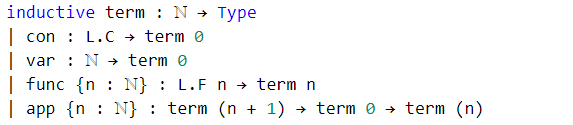
\includegraphics[height=2 in]{termsLean.PNG}
 	\caption{Our definition of term in Lean}

\end{figure}\end{center}

We introduced the notion of 'level' in our definition of terms to account for
functions of various arity and to make it easier to work with recursion in Lean. Let L be a language; then, a (term L n) represents all terms of level n of L. Level 0 terms must be constants, variables, or terms of type L.F 0. Thus, only level 0 terms are L-terms.

\section*{Sentences and Formulae}
We used the definition of formulas and sentences from Marker's \textit{Model Theory}.\\
\textbf{Definition}(Formula): Formulas are finite strings made from the symbols of L,the equality relation =,  variables $x_0$, $x_1$, . . . , the logical connectives $\lnot$ ,$\wedge$,$\lor$,quantifiers $\exists$ and $\forall$ and parentheses.\\

\textbf{Definition}(Free variable / Bound variable):A variable is free in a formula if it is not quantified. Otherwise, this variable is bound.\\


\textbf{Definition}(Sentence):Sentences are formulas with no free variables.\\
\begin{center}\begin{figure}
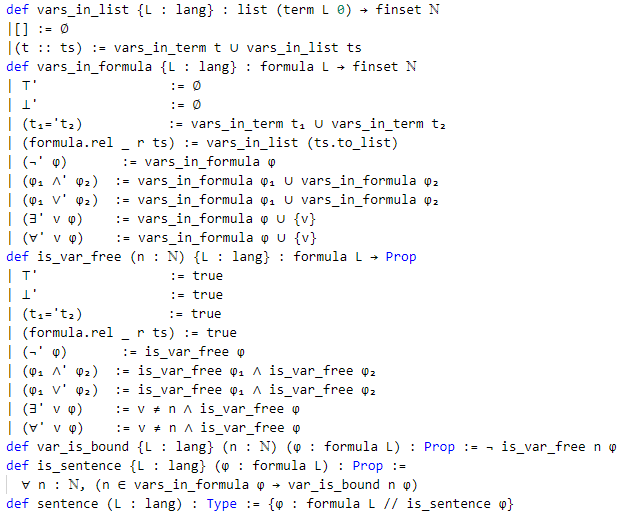
\includegraphics[height = 9 in, width=1\textwidth, left]{sentence.png}
 	\caption{Our definition of sentence in Lean}

\end{figure}\end{center}

We define sentence with the following steps: Firstly, we define helper function vars\_in\_formula to extract variables in formulas. Secondly, we define is\_var\_free and var\_is\_bound to determine whether a given formula is variable free or bound. We then construct the definition of the sentence based on these functions.
\section*{Models}
\end{multicols}


%%%%%%  Here is where the acknowledgements go. If you are in a project which requires additional acknowledgements, add them here
\vfill
 {}\centerline{\emph{
Support for this project was provided by the Illinois Geometry Lab and the Department of Mathematics at the University of Illinois at Urbana-Champaign. We would also like to thank our faculty mentor and our graduate mentors for their support, mentorship and guidance throughout this project.}}


\end{document}







%the boxthm environment automatically puts a box around your theorem
\begin{boxthm}
This didn't have to be a theorem, but could instead refer to a conjecture you've made, or a previous relevant theorem in this area. In lines 66, you can change "Theorem" to "Conjecture" or some other title, that will be used for all statements written in boxthm

If this is a result proven by someone else it's important to cite them in the statement of it.
 \end{boxthm}


%%%%%%%%%%%%%%%%%%%%%%
%% New Column
%%%%%%%%%%%%%%%%%%%%%%%


{\small You can write small text to elaborate on your example if needed. Or wherever else small text might be useful.}


 \begin{minipage}{.5\columnwidth}%this is another way to put text and images side by side
\begin{ex}[Here's a second example]
Here's where you could write about it.
\end{ex}
\end{minipage}
\hspace{7ex}\begin{minipage}{.37\linewidth}
  \begin{center}
%\begin{figure}
%\includegraphics[height=2.25in]{bamboozledagain.jpg}
% 	\caption{Caption goes here}
%\end{figure}
  \end{center}
\end{minipage}

% \section*{Methods and/or Results}
% \subsection*{Name of method/Example:} Here is where you might talk about the methods used in your research, and what obstacles that may have arisen.

% \begin{thm}
% This is a theorem without a box around it, but the same numbering at boxthm.
% You don't need to itemize here, it's just used as an example.
% \begin{itemize}
%     \item First Item
%   \item Second Item
%   \item Third Item
% \end{itemize}
% \end{thm}


% \subsection*{Subsection of your Methods/Results}


% \begin{minipage}{.65\columnwidth}
%   The image file used throughout this poster is called `bamboozledagain.jpg', and must be swapped out for whatever image you choose to use. In order for the image to appear, the image file should be stored in the same folder as your .tex file. Experiment with the relative sizing and placement of images to change up this poster layout.\end{minipage}\hspace{2ex}\begin{minipage}{.3\linewidth}

% \begin{center}\vspace{-2ex}\includegraphics[height=2.5in]{bamboozledagain.jpg}\end{center}\end{minipage}


%  \begin{mdframed}[style=MyFrame]
% % by putting the minipage inside the mdframe, you get a box around the text and image
%  \begin{minipage}{.625\columnwidth}
%  \begin{thm*}
% The use of thm* gives an unnumbered theorem. Look at the difference between line 35 and 36 to see how to do this for conjectures, corollaries, ect.
%  \end{thm*}
%  fdgvoiejmg9uvhrt gu vhdiufhgvdufhgd fvidfjgvdf]dvf
% fdig vjdoifj vodifj vidfjgov idigfdjfg

% \end{minipage}\hspace{1ex}\begin{minipage}{.3\columnwidth}

% \begin{center}\includegraphics[height=3in]{bamboozledagain.jpg}\end{center}\end{minipage}\end{mdframed}


%%%%%%%%%%%%%%%%%%%%%%
%% New Column
%%%%%%%%%%%%%%%%%%%%%%%

\section*{Future Directions }

The next steps in this project would be to formalize
Here is where you can talk about the results of your work going forward

% \subsection{Another Subsection}
% "Lorem ipsum dolor sit amet, consectetur adipiscing elit, sed do eiusmod tempor incididunt ut labore et dolore magna aliqua. Ut enim ad minim veniam, quis nostrud exercitation ullamco laboris."

% \begin{boxthm}
% "Lorem ipsum dolor sit amet, consectetur adipiscing elit, sed do eiusmod tempor incididunt ut labore et dolore magna aliqua. Ut enim ad minim veniam, quis nostrud exercitation ullamco laboris nisi ut aliquip ex ea commodo consequat. Duis aute irure dolor in reprehenderit in voluptate velit esse cillum dolore eu fugiat nulla pariatur. Excepteur sint occaecat cupidatat non proident, sunt in culpa qui officia deserunt mollit anim id est laborum."
%  %\end{theorem}
%  \end{boxthm}

 {\bf {\large Now how might you use this template?}}\vspace{.5ex}
Just because the poster is laid out this way doesn't mean you need to follow its structure down to the spacing: \vspace{1ex}

{\bf Question 1} Experiment! Move the text boxes around, add more or larger pictures. Feel free to change this template up as you make your poster. \vspace{1ex}

{\bf Question 2} Don't know how to do something? Search for it on the internet! A quick search with the right keywords will quickly reveal answers for people who had similar questions.  \vspace{1ex}

{\bf Answering Question 1}. Look at other posters and decide what you liked about them. Walking around the Lab there are plenty of examples of previous IGL posters.

{\bf Answering Question 2}. If you're editing this and something goes wrong don't be afraid to click ctrl+z. We all make mistakes, and that's what it's there for.

\subsubsection*{References}

{\footnotesize [1] Firstname Lastname. A Math Book. \emph{The Secret Society of Mathematical Wonder}, XYZ Press, (2017)

[2] Isaac Riemann. A Proof of Isaac's Hypothesis in Six Pages or Less. \emph{Research Writinigs around Mathematics,} vol. 239, pg 128-133, 1859. }




\end{multicols}
\end{document}
